% !TeX spellcheck = en_GB
% %%% ***************** CHAPTER THEORY ***************** %%%
\chapter{Theory}
\textcolor{red}{\textbf{The overleaf file from the Methodology is here:} \\ \url{https://www.overleaf.com/15461164zgrsztkgnfzd}}
\\
%%%%%%%%%%%%%%%%%%%%%%%%%%%%%%%%%%%%%%%%%%%%%%%%%%%%%%%%%%%%%%%%%%%%%%%%%%
%%%%%%%%%%%%%%%%%%%%%%%%%%%%%%%%%%%%%%%%%%%%%%%%%%%%%%%%%%%%%%%%%%%%%%%%%%

% %%% ***************** CHAPTER IDEAS ***************** %%%
\begin{itemize}
	\item \textbf{Have to think about what I should write here!} \\
		maybe about particle formation (Depositional growth, Riming, Capture nucleation, Aggregation, Ice multiplication, Bergeron-Findeisen process)
%	\item What is attenuation?
%	\item Snow formation and different particles. What was observed at Haukeli?
%	\item Rayleigh scattering \& Radars \citep[p.257, Sec. 9.3.1]{lohmann_introduction_2016}
\end{itemize}
%%%%%%%%%%%%%%%%%%%%%%%%%%%%%%%%%%%%%%%%%%%%%%%%%%%%%%%%%%%%%%%%%%%%%%%%%%
%%%%%%%%%%%%%%%%%%%%%%%%%%%%%%%%%%%%%%%%%%%%%%%%%%%%%%%%%%%%%%%%%%%%%%%%%%

% %%% ***************** EXTRATROPICAL CYCLONE ***************** %%%
% !TeX spellcheck = en_GB
\section{Extratropical Cyclones}\label{sec:ext_cyclone}
%\cite{markowski_mesoscale_2011}
%' midlatitude synoptic-scale motions are arguably solely driven by baroclinic instability; extratropical cyclones are the dominant weather system of midlatitudes on the synoptic scale. Baroclinic instability is most likely to be realized by disturbances.'
%\\
%Extratropical highs and lows have a time-scale of several days and the horizontal extension of several kilometre. \\
%Extratropical cyclones develop with the formation of fronts. \\
%'The destabilization of layers via the potential instability
%mechanism is probably important in the formation
%of mesoscale rainbands within the broader precipitation
%shields of extratropical cyclones on some occasions, especially
%when potentially unstable layers are lifted over a front.
%Potential instability also is often cited as being important
%in the development of deep moist convection.' 'Despite the common presence of
%potential instability, however, it usually does not play a role
%in the destabilization of the atmosphere that precedes the
%initiation of convection.' \\
%'Not only are synoptic fronts and their
%associated baroclinity important for the development of
%larger-scale extratropical cyclones, but in some situations
%evenmesoscale boundaries can influence larger-scale extratropical
%cyclones.' \\
%'In the Norwegian cyclone model, the cold front
%moves faster than the warm front, eventually overtaking
%it, resulting in occlusion of the extratropical cyclone, with
%the occluded front being the surface boundary along which
%the cold front has overtaken the warm front.'

%%%%%%%%%%%%%%%%%%%%%%%%%%%%%%%%%%%%%%%%%%%%%%%%%%%%%%%%%%%%%%%%%%%%%%%%%%
%%%%%%%%%%%%%%%%%%%%%%%%%%%%%%%%%%%%%%%%%%%%%%%%%%%%%%%%%%%%%%%%%%%%%%%%%%



% %%% ***************** SECTION MICROPHY. PROCESSES IN COLD CLOUDS ***************** %%%
% !TeX spellcheck = en_GB
\section{Ice formation} \label{sec:ice_formation}

%%% image double fence @ Haukeli %%%%%%%%%%%%%%%%%%%%%%%%%%%%%%%%%%%%%
% !TeX spellcheck = en_GB
\begin{figure}
	\centering
	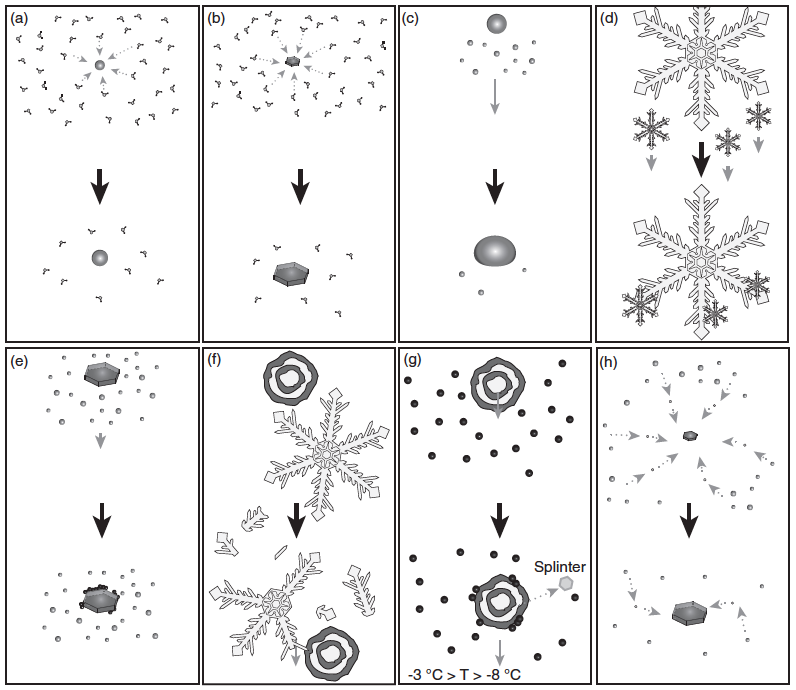
\includegraphics[width=\textwidth]{./fig_theory/Lohman_growing}
	\caption{\cite{lohmann_introduction_2016} }\label{fig:ice_growth}
\end{figure}
%%%%%%%%%%%%%%%%%%%%%%%%%%%%%%%%%%%%%%%%%%%%%%%%%%%%%%%%%%%%%%%%%%%%%%%%%%

%\section{Bergeron-Findeisen effect}

%%%%%%%%%%%%%%%%%%%%%%%%%%%%%%%%%%%%%%%%%%%%%%%%%%%%%%%%%%%%%%%%%%%%%%%%%%
%%%%%%%%%%%%%%%%%%%%%%%%%%%%%%%%%%%%%%%%%%%%%%%%%%%%%%%%%%%%%%%%%%%%%%%%%%